\chapter{Deep Learning}
\thispagestyle{chapterfancy}

Deep Neural Networks are a type of machine learning model that are considered, as of the time of writing, the most powerful and practical machine learning models, with applications in computer vision, speech recognition, natural language processing, and many more. \\
Machine learning models can be coarsely be divided into three areas: supervised, unsupervised, and reinforcement learning. In this thesis we will focus solely on the Supervised Deep Learning. \\
To be able to properly explain the importance and power of Deep Neural Networks, we will utilize as reference the book "Understanding Deep Learning" by Simon J.D. Prince \cite{prince2024understanding}. 

\section{Supervised Learning}
 
In supervised learning, we aim to build a model that takes an input $x$ and outputs a prediction $y$, while using a labeled dataset, where the input data is paired with corresponding output labels. To make the prediction, we need a model $f[\bullet]$ that takes input $x$ and returns $y$. The model is just a mathematical equation with a fixed form that contains parameters $\phi$, which determine the particular relation between input and output. When we talk about learning or training a model, we mean that we attempt to find parameters that make sensible output predictions from the input. We learn these parameters using a training dataset of $I$ pairs of input and output examples $\{x_{i}, y_{i}\}$. We aim to select parameters that map each training input to its associated output as closely as possible. We quantify the degree of mismatch in this mapping with the loss $L$, a scalar value that summarizes how poorly the model predicts the training outputs
from their corresponding inputs for parameters $\phi$. When we train the model, we are seeking parameters $\hat{\phi}$ that minimize this loss function:

\begin{equation}
    \hat{\phi}=\underset{\phi}{\text{argmin}}\Bigl[L[\{x_{i},y_{i}\},\phi]\Bigr]
\end{equation}

\noindent After training a model, we run the model on separate test data to see how well it generalizes to examples that it didn't observe during training. If the performance is adequate, then we are ready to deploy the model.

\section{Shallow Neural Networks}
Shallow neural networks are functions $y = f[x, \phi]$ with parameters $\phi$ that map a multi-dimensional input $x \in \mathbb{R}^{D_{i}}$ to a multi-dimensional output $y \in \mathbb{R}^{D_{o}}$ using $h \in \mathbb{R}^{D}$ hidden units. Each hidden unit is computed as:

\begin{equation}
    h_{d}=a\left[\theta_{d0}+\sum_{i=1}^{D_{i}} \theta_{d i} x_{i}\right]
\end{equation}

\noindent and these are combined linearly to create the output:

\begin{equation}
    y_{j}=\phi_{j0}+\sum_{d=1}^{D} \phi_{j d} h_{j}
\end{equation}

\noindent where $a[\bullet]$ is a nonlinear activation function. The activation function permits the model to describe nonlinear relations between input and the output, and as such, it must be nonlinear itself; with no activation function, or a linear activation function, the overall mapping from input to output would be restricted to be linear. Figure \ref{fig:ShallowNet} shows an example with three inputs, three hidden units, and two outputs. \\

\begin{figure}[H]
    \centering
    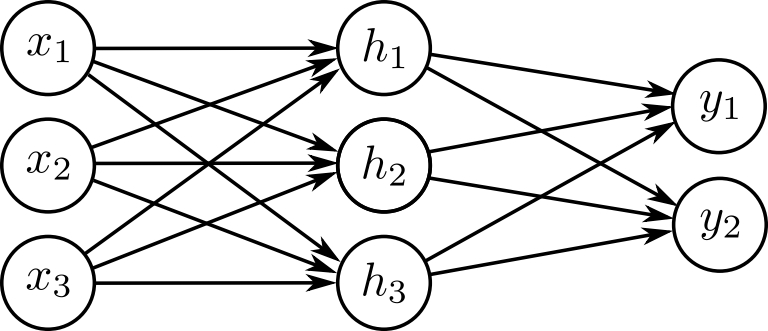
\includegraphics[width=0.6\linewidth]{Images/ShallowNetThreeInputsTwoOutputs.jpg}
    \caption{Visualization of neural network with three inputs and two outputs.}
    \label{fig:ShallowNet}
\end{figure}

\noindent Many different activation functions exist in the literature; Figure \ref{fig:ShallowActivations} illustrates the most common ones, which we will not get into much detail in this thesis. The most common one is the Rectified linear unit (ReLU, Figure \ref{fig:ShallowReLU}), which has the merit of being easily interpretable:

\begin{equation}
    \text{ReLU}\left[ z\right] =\begin{cases}0 \quad z<0 \\ z \quad z \geq 0\end{cases}
\end{equation}

\noindent With ReLU activations, the network divides the input space into convex polytopes where all points in the same linear region activate the same nodes. Each convex polytope contains a different linear function. The polytopes are the same for each output node, but the linear functions they contain can differ. For more information about these linear regions, consult \cite{zhang2020empirical}.

\begin{figure}[H]
    \centering
    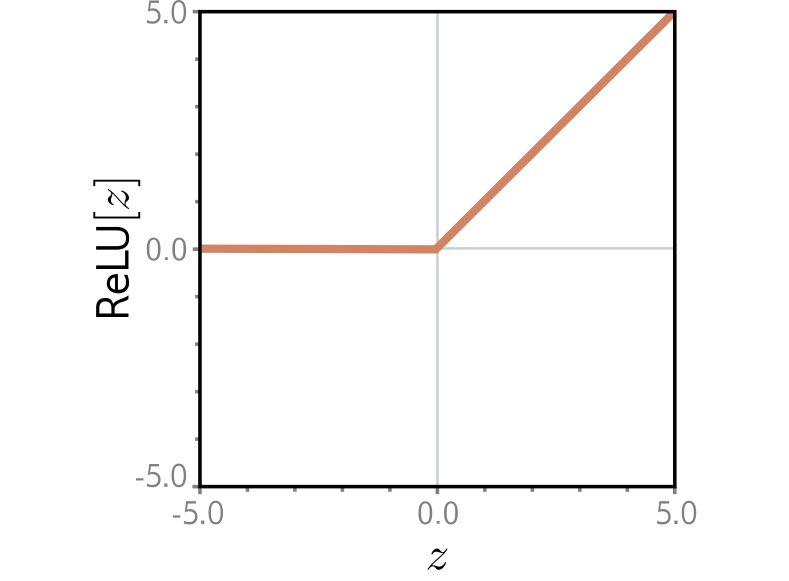
\includegraphics[width=0.7\linewidth]{Images/ShallowReLU.jpg}
    \caption{Rectified linear unit (ReLU).}
    \label{fig:ShallowReLU}
\end{figure}

\begin{figure}[H]
    \centering
    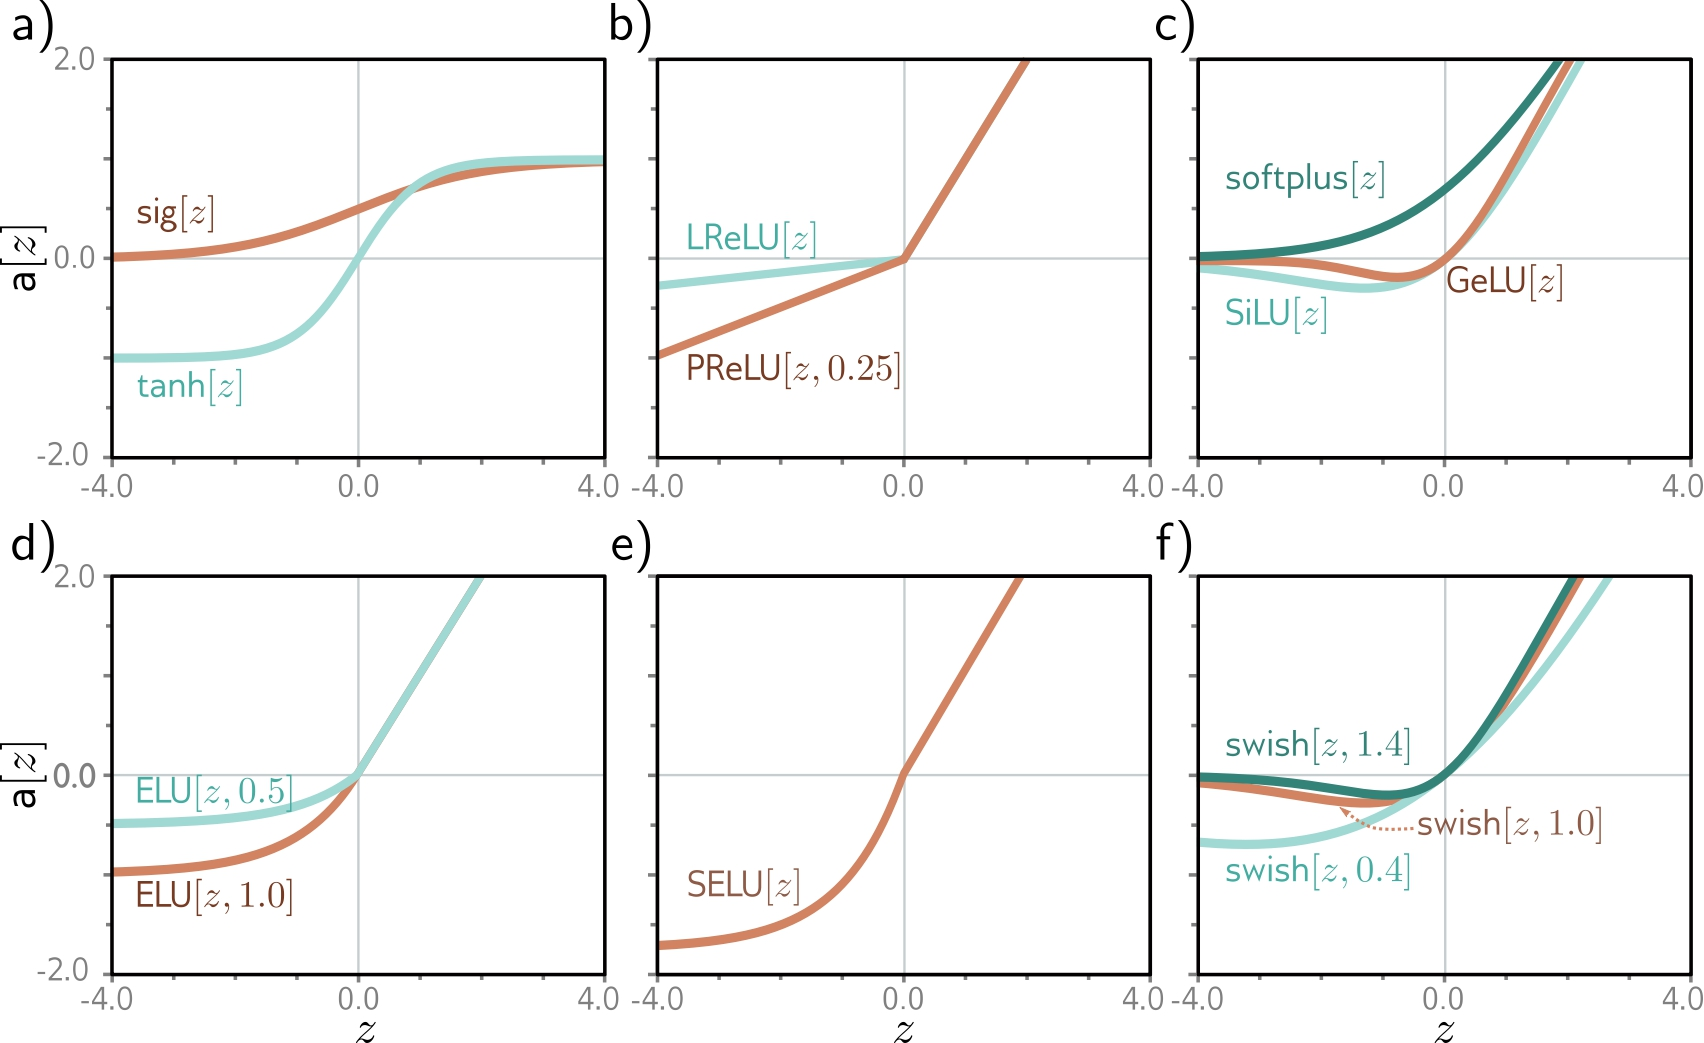
\includegraphics[width=0.95\linewidth]{Images/ShallowActivations.jpg}
    \caption{Activation functions. a) Logistic sigmoid and tanh functions. b) Leaky ReLU and parametric ReLU with parameter 0.25. c) SoftPlus, Gaussian error linear unit, and sigmoid linear unit. d) Exponential linear unit with parameters 0.5 and 1.0, e) Scaled exponential linear unit. f) Swish with parameters 0.4, 1.0, and 1.4.}
    \label{fig:ShallowActivations}
\end{figure}

\pagebreak 

\section{Deep Neural Networks}
As the number of hidden units increases, shallow neural networks improve their descriptive power. Indeed, with enough hidden units, shallow networks can describe arbitrarily complex functions in high dimensions. However, it turns out that for some functions, the required number of hidden units is impractically large. Deep networks can produce many more linear regions than shallow networks for a given number of parameters. Hence, from a practical standpoint, they can be used to describe a broader family of functions. Modern networks might have more than a hundred layers with thousands of hidden units at each layer. The number of hidden units in each layer is referred to as the width of the network, and the number of hidden layers as the depth. The total number of hidden units is a measure of the network’s capacity.

\begin{figure}[H]
    \centering
    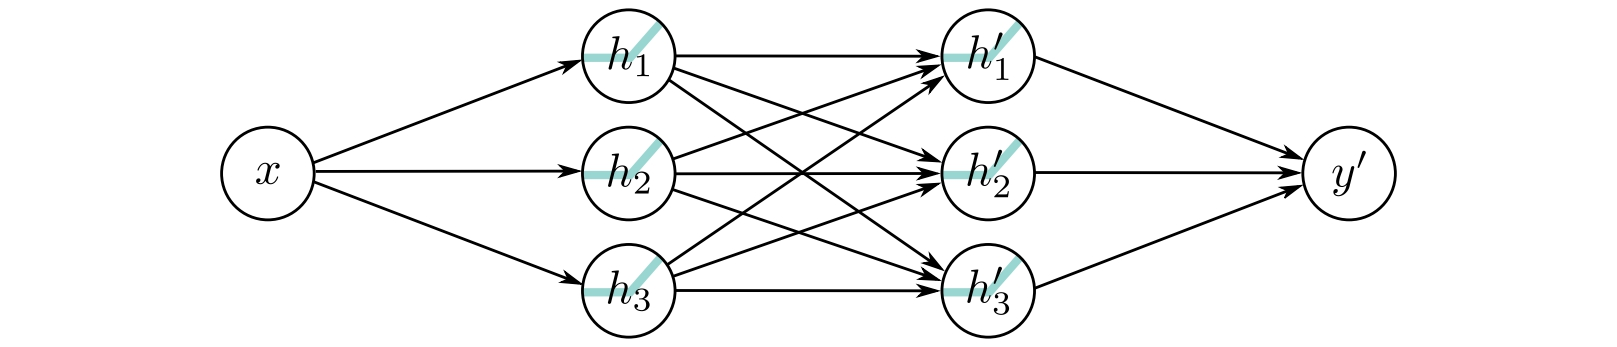
\includegraphics[width=0.9\linewidth]{Images/DeepTwoLayer.jpg}
    \caption{Neural network with one input, one output, and two hidden layers, each containing three hidden units.}
    \label{fig:DeepNet}
\end{figure}

\noindent In the general case of a deep network with input $x \in \mathbb{R}^{D_{0}}$, output $y \in \mathbb{R}^{D_{out}}$, depth $n$ and $h_{k} \in \mathbb{R}^{D_{k}}$ hidden units at depth $k$, the hidden layers are defined by:

\begin{equation}
    h_{k, d}=a\left[\theta_{k, d0}+\sum_{i=1}^{D_{k-1}} \theta_{k, d i} h_{k-1, d}\right]
\end{equation}

\noindent while the output is computed as follows:

\begin{equation}
    y_{j}=\phi_{j0}+\sum_{d=1}^{D_{n-1}} \phi_{j d} h_{n-1,j}
\end{equation}

\noindent Both deep and shallow networks can model arbitrary functions, but some functions can be approximated much more efficiently with deep networks. Functions have been identified that require a shallow network with exponentially more hidden units to achieve an equivalent approximation to that of a deep network. This phenomenon is referred to as the depth efficiency of neural networks.

\section{Loss Functions}
A loss function or cost function $L[\{x_{i},y_{i}\},\phi]$ returns a single number that describes the mismatch between the model predictions $f[x_{i}, \phi]$ and their corresponding ground-truth outputs $y_{i}$. During training, we seek parameter values $\phi$ that minimize the loss and hence map the training inputs to the outputs as closely as possible.

\subsection{Cross-Entropy Loss}
The cross-entropy loss is based on the idea of finding parameters $\theta= (\mu, \sigma^{2})$ that minimize the distance between the empirical distribution $q(y)$ of the observed data $y$ and a model distribution $P_{r}(y|\theta)$ (figure \ref{fig:LossCrossEntropy}). The distance between two probability distributions $q(z)$ and $p(z)$ can be evaluated using the Kullback-Leibler divergence (Section \ref{ch:KLD}):

\begin{equation}
    D_{KL}[q \| p] = \int_{-\infty}^{+\infty} q(z) \log [q(z)] d z-\int_{-\infty}^{+\infty} q(z) \log [p(z)] d z
\end{equation}

\noindent Now consider that we observe an empirical data distribution at points $\{y_{i}\}^{I}_{i=1}$. We can describe this as a weighted sum of point masses:

\begin{equation}
    q(y)=\frac{1}{I} \sum_{i=1}^{I} \delta\left[y-y_{i}\right]
    \label{eq:EmpiricalDistribution}
\end{equation}

\noindent where $\delta[\bullet]$ is the Dirac delta function (Section \ref{ch:Dirac}). We want to minimize the KL divergence between the model distribution $Pr(y|\theta)$ and this empirical distribution:

\begin{equation}
\begin{aligned}
    \hat{\theta} & = \underset{\theta}{\text{argmin}}\left[\int_{-\infty}^{+\infty} q(y) \log [q(y)] d y-\int_{-\infty}^{+\infty} q(y) \log [Pr(y|\theta)] dy\right] \\
    & = \underset{\theta}{\text{argmin}}\left[-\int_{-\infty}^{+\infty} q(y) \log [Pr(y|\theta)] d y\right]
\end{aligned}
\end{equation}

\noindent where the first term disappears, as it has no dependence on $\theta$. The remaining second term is known as the cross-entropy, which can be interpreted as the amount of uncertainty that remains in one distribution after taking into account what we already know from the other. Now, we substitute in the definition of $q(y)$ from equation \ref{eq:EmpiricalDistribution}:

\begin{equation}
\begin{aligned}
    \hat{\theta} 
    & = \underset{\theta}{\text{argmin}}\left[-\int_{-\infty}^{+\infty} \left(\frac{1}{I} \sum_{i=1}^{I} \delta\left[y-y_{i}\right]\right) \log [Pr(y|\theta)] d y\right] \\
    & = \underset{\theta}{\text{argmin}}\left[-\frac{1}{I} \sum_{i=1}^{I}log[Pr(y_{i}|\theta)]\right] \\
    & = \underset{\theta}{\text{argmin}}\left[-\sum_{i=1}^{I}log[Pr(y_{i}|\theta)]\right]
\end{aligned}
\end{equation}

\noindent In machine learning, the distribution parameters $\theta$ are computed by the model $f[x_{i}, \phi]$, so we have:

\begin{equation}
    \hat{\phi} = \underset{\phi}{\text{argmin}}\left[-\sum_{i=1}^{I}log\Bigl[Pr(y_{i}|f[x_{i}, \phi])\Bigr]\right]
\end{equation}

\noindent with the softmax function (Section \ref{ch:Softmax}) as the probability:

\begin{equation}
    Pr(y_{i}|f[x_{i}, \phi]) = \text{softmax}_{y_{i}}\Bigl[f[x_{i}, \phi]\Bigr] = \frac{\exp \Bigl[f_{y_{i}}[x_{i}, \phi]\Bigr]}{\sum_{k=1}^{I} \exp \Bigl[f_{k}[x_{i}, \phi]\Bigr]}
\end{equation}

\noindent where $f_{k}[x, \phi]$ denotes the $k^{th}$ output of the neural network.

\begin{figure}[H]
    \centering
    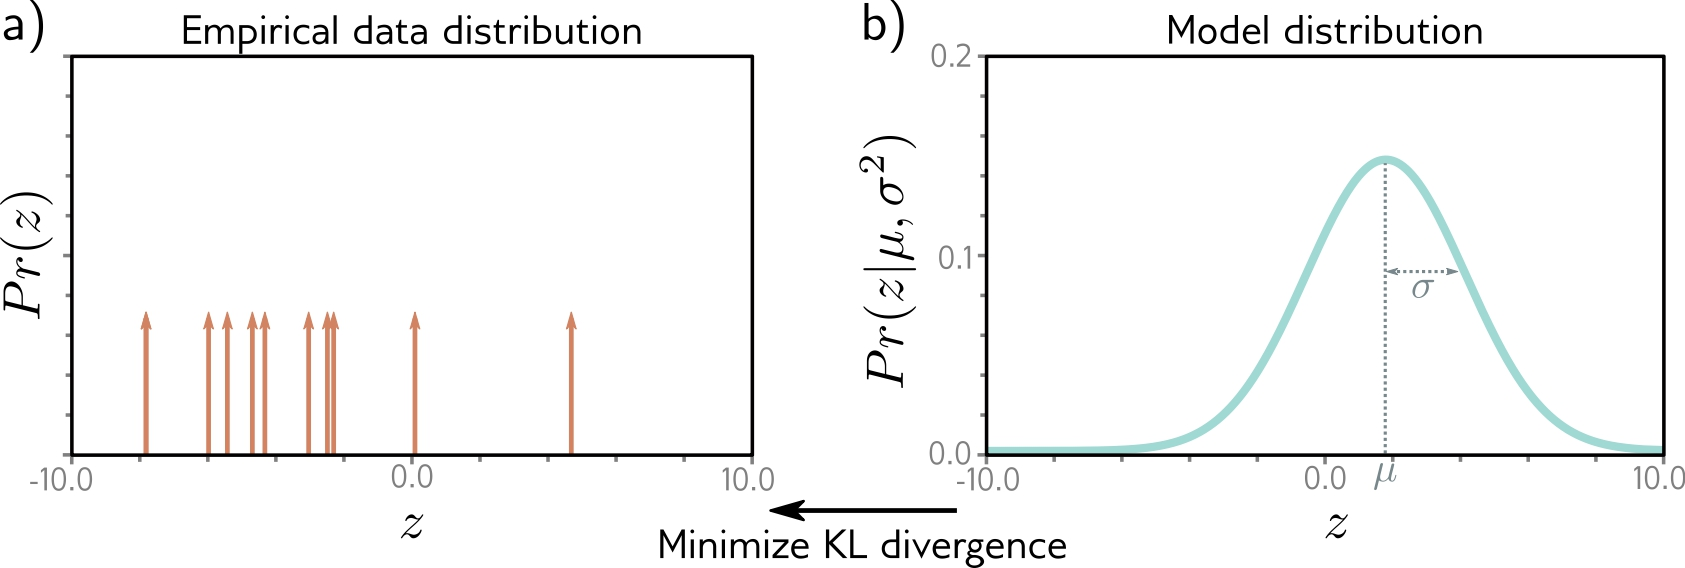
\includegraphics[width=0.9\linewidth]{Images/LossCrossEntropy.jpg}
    \caption{Cross-entropy method. a) Empirical distribution of training samples (arrows denote Dirac delta functions). b) Model distribution (a normal distribution with parameters $\theta = \mu, \sigma^{2}$).}
    \label{fig:LossCrossEntropy}
\end{figure}

\subsection{Contrastive Learning}
The idea behind contrastive learning is to learn a function that encodes the input into an embedding vector such that samples from the same class have similar embeddings while samples from different classes have very different ones. The most common usage of this idea is self-supervised contrastive learning, where an anchor gets compared to a single positive, which usually is an augmented version of the anchor (\textit{i.e.}, a modified or transformed variant of the original sample, created through techniques like rotation, flipping, or scaling), and a set of negatives, consisting of the remainder of the batch. \\
A novel interpretation of this idea has been proposed by Khosla \textit{et al.} called "Supervised Contrastive Learning" \cite{khosla2020supervised}. This approach contrasts the set of all samples from the same class as positives against the negatives from the remainder of the batch, as shown in Figure \ref{fig:SelfConVSSupCon}.

\begin{figure}[H]
    \centering
    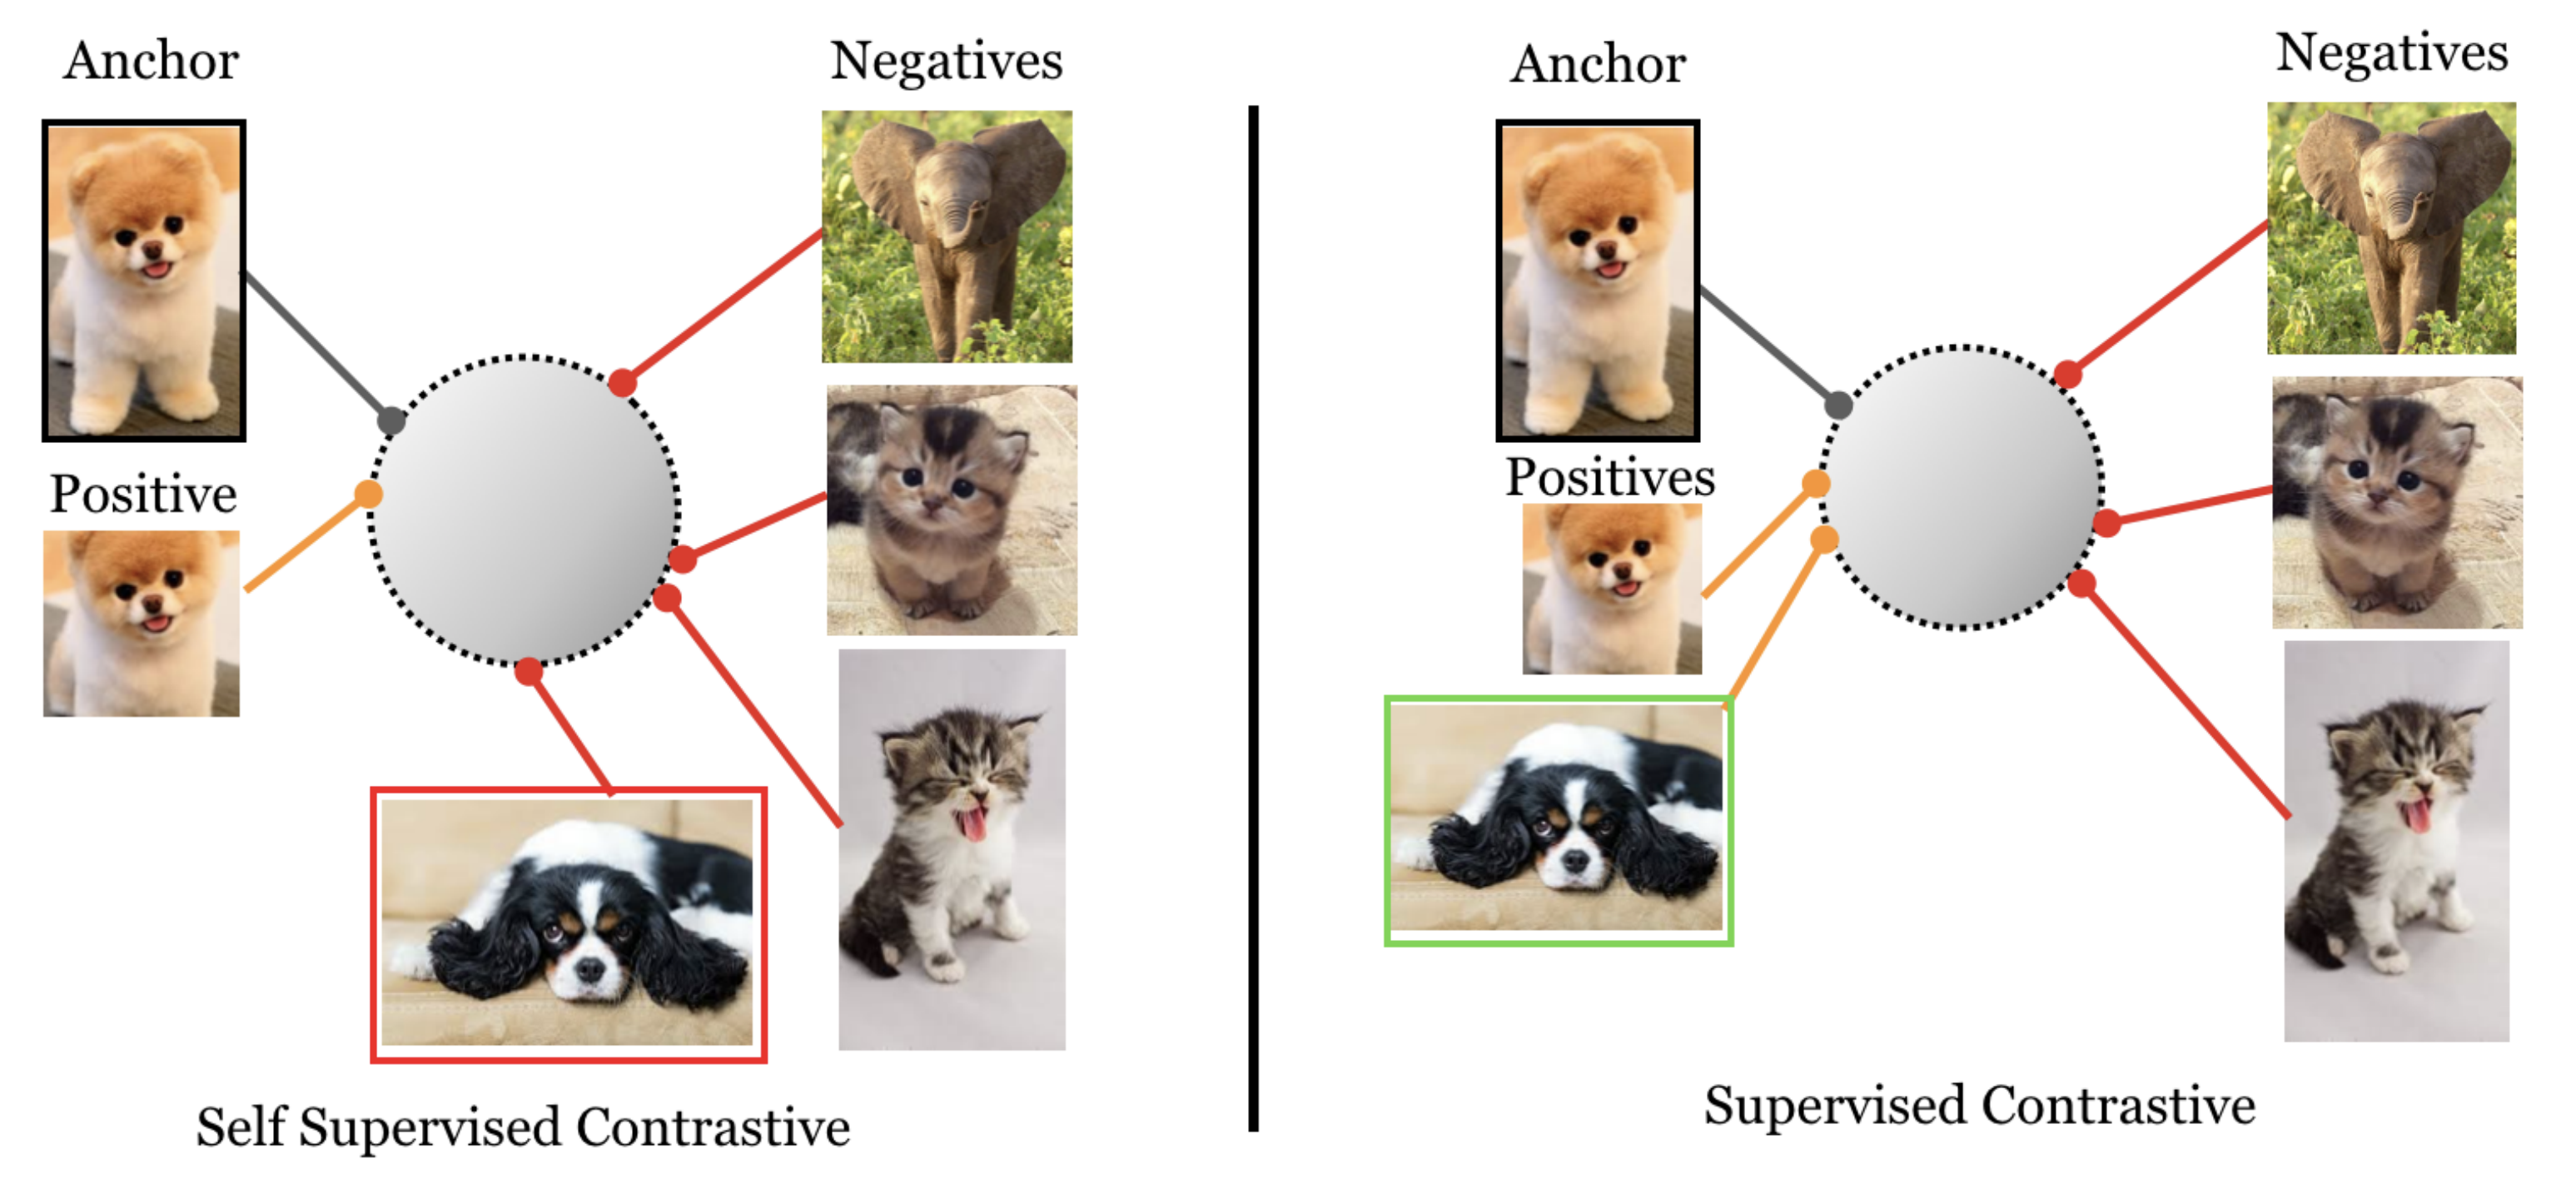
\includegraphics[width=0.9\linewidth]{Images/SelfConVSSupCon.png}
    \caption{Supervised vs. self-supervise contrastive loss.}
    \label{fig:SelfConVSSupCon}
\end{figure}

\subsubsection{Self-supervised Contrastive Loss}
Within a batch, let $i \in I \equiv {1,...,N}$ be the index of an arbitrary sample, and let $j(i)$ be the index of the augmented sample. In self-supervised contrastive learning, the loss takes the following form:

\begin{equation}
    \mathcal{L}^{\text {self}}=\sum_{i \in I} \mathcal{L}_{i}^{\text {self}} = -\sum_{i\in I} \log \frac{\exp \left(v_{i} \cdot v_{j(i)} / \tau\right)}{\sum_{a\in A(i)} \exp \left(v_{i} \cdot v_{a} / \tau\right)}
\end{equation}

\noindent where $v_{i}$ represents the embedding of the input $x_{i}$, $\tau\in\mathbb{R}^{+}$ is a scalar temperature parameter and $A(i)\equiv I\backslash\{i\}$.

\subsubsection{Supervised Contrastive Loss}
Within a batch, let $i \in I \equiv {1,...,N}$ be the index of an arbitrary sample. In supervised contrastive learning, the loss takes the following form:

\begin{equation}
    \mathcal{L}^{\text {sup }}=\sum_{i \in I} \mathcal{L}_{i}^{\text {sup}} =\sum_{i \in I} \frac{-1}{|P(i)|} \sum_{p\in P(i)} \log \frac{\exp \left(v_{i} \cdot v_{p} / \tau\right)}{\sum_{a\in A(i)} \exp \left(v_{i} \cdot v_{a} / \tau\right)}
\end{equation}

\noindent where $v_{i}$ represents the embedding of the input $x_{i}$, $\tau\in\mathbb{R}^{+}$ is a scalar temperature parameter, $A(i)\equiv I\backslash\{i\}$, $P(i)\equiv \{p\in A(i) : l_{p} = l_{i}\}$ is the set of indices of all positives in the batch apart from $i$ ($l_{i}$ is the label of $x_{i}$) and $|P(i)|$ is its cardinality. It uses the positive normalization factor (\textit{i.e.}, $\frac{1}{|P(i)|}$) to remove bias present in multiple positives samples and preserve the summation over negatives in the denominator to increase performance.

\section{Fitting models}
Finding the parameters that minimize this loss as learning the network’s parameters or simply as training or fitting the model. The process is to choose initial parameter values and then iterate the following two steps: (i) compute the derivatives (gradients) of the loss with respect to the parameters, and (ii) adjust the parameters based on the gradients to decrease the loss. After many iterations, we hope to reach the overall minimum of the loss function.

\subsection{Gradient Descent}
The goal of an optimization algorithm is to find parameters $\hat{\phi}$ that minimize the loss:

\begin{equation}
    \hat{\phi}=\underset{\phi}{\text{argmin}}\Bigl[L[\phi]\Bigr]
\end{equation}

\noindent The simplest method in this class is gradient descent. This starts with initial parameters $\phi = [\phi_{0}, \phi_{1}, . . . , \phi_{N} ]^{T}$ and iterates two steps:

\begin{itemize}
    \item \textbf{Step 1.} Compute the derivatives of the loss with respect to the parameters:

    \begin{equation}
        \frac{\partial L}{\partial \phi}=\left[\begin{array}{c}\frac{\partial L}{\partial \phi_{0}} \\ \frac{\partial L}{\partial \phi_{1}} \\ \vdots \\ \frac{\partial L}{\partial \phi_{N}}\end{array}\right]
    \end{equation}

    \item \textbf{Step 2.} Update the parameters according to the rule:

    
    \begin{equation}
        \phi \longleftarrow \phi - \alpha \cdot \frac{\partial L}{\partial \phi}
    \end{equation}
\end{itemize}

\noindent where the positive scalar $\alpha$ determines the magnitude of the change. The parameter $\alpha$ may be fixed (in which we call it a learning rate), or we may perform a line search where we try several values of $\alpha$ to find the one that most decreases the loss. At the minimum of the loss function the gradient will be zero, and the parameters will stop changing. In practice, we monitor the gradient magnitude and terminate the algorithm when it becomes too small.

\subsection{Stochastic Gradient Descent}
Using gradient descent to find the global optimum of a high-dimensional loss function is challenging. We can find a minimum, but there is no way to tell whether this is the global minimum or even a good one. One of the main problems is that the final destination of a gradient descent algorithm is entirely determined by the starting point. Stochastic gradient descent (SGD) attempts to remedy this problem by adding some noise to the gradient at each step. \\
The mechanism for introducing randomness is simple. At each iteration, the algorithm chooses a random subset of the training data and computes the gradient from these examples alone. The update rule for the model parameters $\phi_{t}$ at iteration $t$ is hence:

\begin{equation}
    \phi_{t+1} \longleftarrow \phi_{t}-\alpha \cdot \sum_{i \in \mathcal{B}_{t}} \frac{\partial \ell_{i}\left[\phi_{t}\right]}{\partial \phi}
\end{equation}

\noindent where $\mathcal{B}_{t}$ is a set containing the indices of the input/output pairs in the current batch and, as before, $l_{i}$ is the loss due to the $i^{th}$ pair. The algorithm works through the training examples until it has used all the data, at which point it starts sampling from the full training dataset again. A single pass through the entire training dataset is referred to as an epoch. \\
SGD has several attractive features:
\begin{enumerate}
    \item although it adds noise to the trajectory, it still improves the fit to a subset of the data at each iteration. Hence, the updates tend to be sensible even if they are not optimal.
    \item because it draws training examples without replacement and iterates through the dataset, the training examples all still contribute equally.
    \item it is less computationally expensive to compute the gradient from just a subset of the training data.
    \item it can (in principle) escape local minima.
    \item it reduces the chances of getting stuck near saddle points
\end{enumerate}

\noindent There is also some evidence that SGD finds parameters for neural networks that cause them to generalize well to new data in practice.

\subsection{Momentum}
A common modification to stochastic gradient descent is to add a momentum term. We update the parameters with a weighted combination of the gradient computed from the current batch and the direction moved in the previous step:

\begin{equation}
    \begin{aligned}
    & m_{t+1} \longleftarrow \beta \cdot m_{t}+(1-\beta) \sum_{i \in B_{t}} \frac{\partial l_{i}\left[\phi_{t}\right]}{\partial \phi} \\ 
    & \phi_{t+1} \longleftarrow \phi_{t}-\alpha \cdot m_{t+1}
    \end{aligned}
\end{equation}

\noindent where $m_{t}$ is the momentum (which drives the update at iteration $t$), $\beta \in [0, 1)$ controls the degree to which the gradient is smoothed over time, and $\alpha$ is the learning rate. \\
The recursive formulation of the momentum calculation means that the gradient step is an infinite weighted sum of all the previous gradients, where the weights get smaller as we move back in time. The effective learning rate increases if all these gradients are aligned over multiple iterations but decreases if the gradient direction repeatedly changes as the terms in the sum cancel out. The overall effect is a smoother trajectory and reduced oscillatory behavior in valleys.

\section{Residual Neural Networks}
Residual neural networks (ResNets) are an innovative type of deep neural network architecture that introduces residual blocks, proposed by He \textit{et al.} \cite{he2016deep}. \\
Every network that came before this processed the data sequentially, \textit{i.e.} each layer receives the previous layer’s output and passes the result to the next. In principle, we could add as many layers as we wanted to, however image classification performance decreased as further layers were added. To solve this, ResNets were presented. Here, each network layer computes an additive change to the current representation instead of transforming it directly. This allows deeper networks to be trained and improve performance across a variety of tasks. \\
In ResNets, each residual block contains a batch normalization operation, a ReLU activation function, and a convolutional layer.

\subsection{Residual Connections and Residual Blocks}
Let’s focus on a local part of a neural network, as depicted in Figure \ref{fig:ResBlock}. Denote the input by $x$. We assume that $f(x)$, the desired underlying mapping we want to obtain by learning, is to be used as input to the activation function on the top. On the left, the portion within the dotted-line box must directly learn $f(x)$. On the right, the portion within the dotted-line box needs to learn the residual mapping $g(x)=f(x)-x$, which is how the residual block derives its name. If the identity mapping $f(x)=x$ is the desired underlying mapping, the residual mapping amounts to $g(x)=0$ and it is thus easier to learn: we only need to push the weights and biases of the upper weight layer (e.g., fully connected layer and convolutional layer) within the dotted-line box to zero. The right figure illustrates the residual block of ResNet, where the solid line carrying the layer input $x$ to the addition operator is called a residual connection (or shortcut connection). With residual blocks, inputs can forward propagate faster through the residual connections across layers. In fact, the residual block can be thought of as a special case of the multi-branch Inception block: it has two branches one of which is the identity mapping.

\begin{figure}[H]
    \centering
    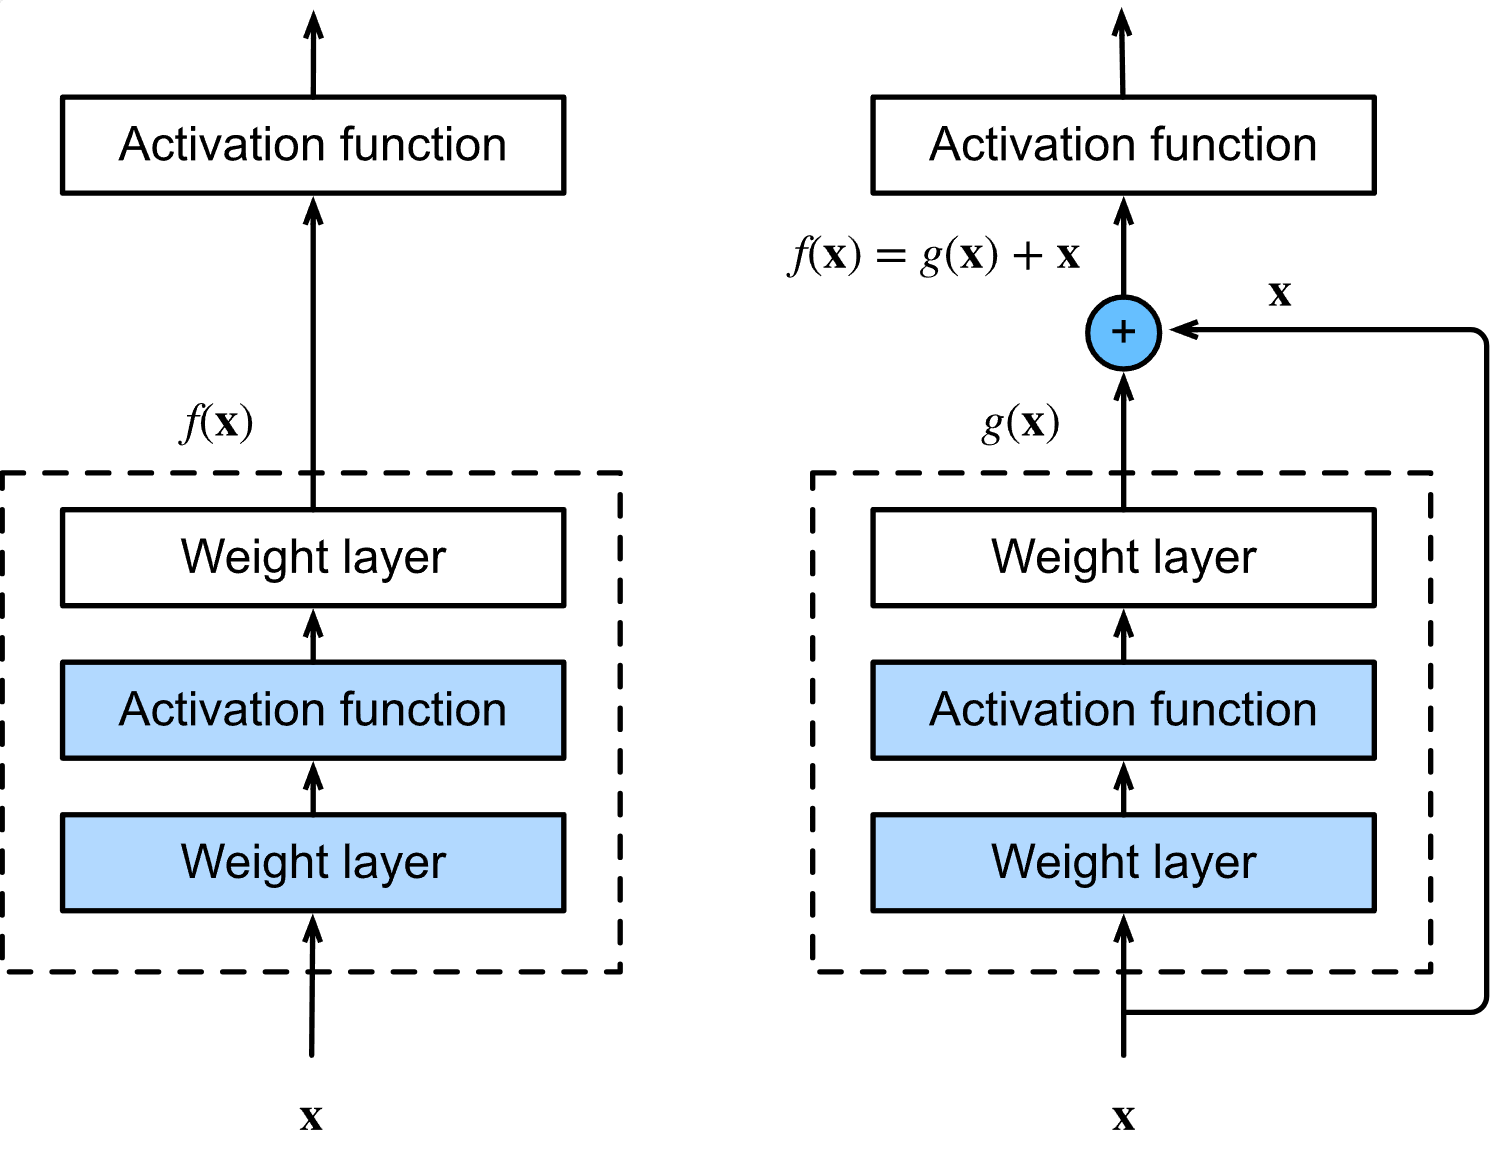
\includegraphics[width=0.7\linewidth]{Images/ResBlock.png}
    \caption{In a regular block (left), the portion within the dotted-line box must directly learn the mapping $f(x)$. In a residual block (right), the portion within the dotted-line box needs to learn the residual mapping $g(x)=f(x)-x$, making the identity mapping $f(x)=x$ easier to learn.}
    \label{fig:ResBlock}
\end{figure}

\subsection{Batch Normalization}
Batch normalization or BatchNorm is a technique, introduced by Sergey Ioffe and Christian Szegedy \cite{ioffe2015batch}, to mitigate the internal covariate shift problem, \textit{i.e.} the change in the distribution of network activations due to the change in network parameters during training. \\
Standardizing our data before entering training is essential for any model we’re building and BatchNorm makes sure data continues to stay scaled while it’s training. \\
Since the full whitening of each layer’s inputs is costly and not everywhere differentiable, they make two necessary simplifications:
\begin{enumerate}
    \item they normalize each scalar feature independently, by making it have the mean of 0 and the variance of 1. Note that simply normalizing each input of a layer may change what the layer can represent, so, to address this, they make sure that the transformation inserted in the network can represent the identity transform by introducing a pair of learnable parameters $\lambda$ and $\beta$ which scale and shift the normalized value.
    \item in the batch setting where each training step is based on the entire training set, we would use the whole set to normalize activations, which is impractical when using stochastic optimization. To simplify this, since mini-batches are used in stochastic gradient training, each mini-batch produces estimates of the mean and variance of each activation. This way, the statistics used for normalization can fully participate in the gradient backpropagation.
\end{enumerate}

\noindent The full algorithm for Batch normalization is presented below.

\begin{figure}[H]
    \centering
    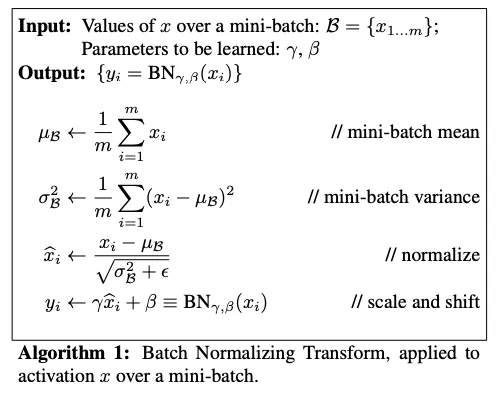
\includegraphics[width=0.65\linewidth]{Images/BatchNorm.png}
    \label{fig:BatchNorm}
\end{figure}

\subsection{Convolutional Layer}
A convolutional layer comprises a set of filters (or kernels), smaller than the input image, with trainable parameters. During training, each filter slides across the height and width of the image, computing the dot product with the input at every spatial position. This process generates an activation map for each filter. In the convolution process (shown in Figure \ref{fig:ConvLayer}), the first entry of the activation map corresponds to the convolution of the filter with a specific region in the input image. This pattern repeats for every element in the input, producing the complete activation map. The output volume of the convolutional layer is formed by stacking the activation maps of all filters along the depth dimension. Each component of an activation map can be seen as the output of a neuron. Neurons are locally connected to small regions in the input image, with the region's size matching the filter size. Moreover, all neurons within an activation map share parameters. This local connectivity forces the network to learn filters that respond maximally to specific local regions in the input. The convolutional layers' design dictates that initial layers capture low-level features like lines, while subsequent layers extract higher-level features such as shapes and specific objects. This hierarchical approach enables the network to progressively learn and represent complex features in images. A padding may be applied to the input image to prevent it from reducing its dimensions after applying the filter.

\begin{figure}[H]
    \centering
    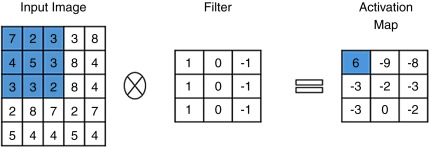
\includegraphics[width=0.7\linewidth]{Images/ConvLayer.png}
    \caption{A graphical example of the convolution process.}
    \label{fig:ConvLayer}
\end{figure}

\subsection{ResNet18}
ResNet18 is the 18 layer version of the Residual Neural Network proposed by He \textit{et al.} \cite{he2016deep}. The base version takes as input a 224*224*3 image, \textit{i.e.} a 224*224 RGB image. The first layer is a Convolutional Layer with 64 kernels 7x7 with a stride of 2 and a padding of 3. This changes the dimension of the input to a 112*112*64. Then, a maxpool  with kernel 3x3, a stride of 2 and padding of 1 is applied, which halves the dimension of the input again, making it a 56*56*64. The Network is divided in 4 main groups (Layer $1\sim4$ in Figure \ref{fig:ResNet}).

\begin{itemize}
    \item \textbf{Layer 1.} Four Residual Blocks are applied to the network, with two skip connections after the second and the fourth. Each block has a convolutional layer with 64 3x3 kernel, a stride of 1, and a padding of 1. After applying all the Blocks, our input will maintain its dimension of 56*56*64.
    \item \textbf{Layer 2/3/4.} Four Residual Blocks are applied to the network, with two skip connections after the second and the fourth. Each block has a convolutional layer with 128/256/512 3x3 kernels, the first one with a stride of 2 and a padding of 1, while the other three with a stride of 1 and a padding of 1. The first skip connection will also feature an identity downsample (\textit{i.e.}, a convolutional layer of 128/256/512 1x1 kernels, with stride of 2 and no padding, followed by a BatchNorm, that reduces the dimension of the input to be able to apply the sum after the skip connection). After applying all the Blocks, our input will have its dimension reduced to 28*28*128/14*14*256/7*7*512.
\end{itemize}

\noindent Finally, an avgpool is applied to the output of Layer 4, to obtain as output a vector of length 512. The last linear layer is optional, depending if want we want our output to be an embedding (no linear layer) or a classification.

\begin{figure}[H]
    \centering
    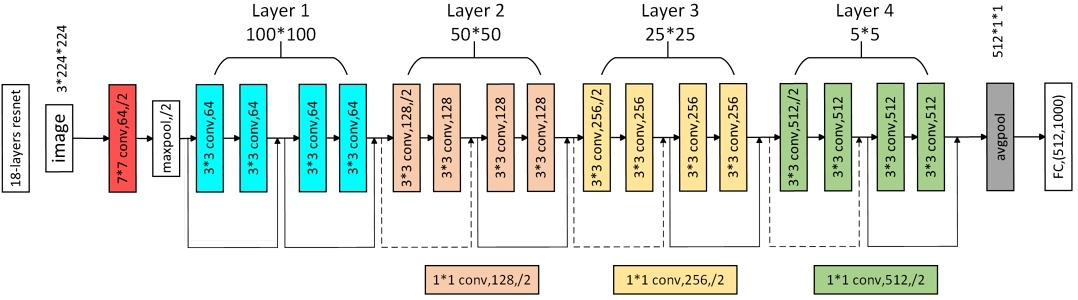
\includegraphics[width=\linewidth]{Images/ResNet.png}
    \caption{A visual explanation of the ResNet18 architecture.}
    \label{fig:ResNet}
\end{figure}